\chapter{Design}

\section{Introduction} % (fold)
\label{sec:introduction}

Today the web has become the central point of all applications. With the presence of Internet, users can use many applications without the need to 
install the program on their machine. Technologies such as JavaScript, HTML, CSS are evolving rapidly and have created the opportunity for the users of 
world wide web to have a more pleasant experience. Fast and robust applications play an important role in attracting users and convincing them to 
migrate from installing the programs on their machine to using their browsers instead. In order to build the most solid web applications possible, 
it is in our best interest to implement new, state of the art software engineering designs.

\subsection{Purpose} % (fold)
\label{sub:purpose}

This chapter describes the architecture design of the AssisTU application. It is intended to describe the design of the system 
thoroughly enough to allow future contributors of the project to clearly understand of how the software is expected to be extended. It will provide 
an overview and description of the system, the relations between the components and user interactions. 

\subsection{Scope} % (fold)
\label{sub:scope}
The scope of the AssisTU software design is set to a basic system that illustrates a proof of concept. Its purpose is the act of writing 
scientific articles that provides planning, organizing tasks, discussions and suggestions.

\section{Use Cases} % (fold)
\label{sec:system_overview}
\subsection{Actors} % (fold)
\label{sub:actors}
\subsubsection{Student/Researcher User} 
The Student/Researcher user is the main user of the application. This user can make extensive use of all the features provided by the application. 
For example, the Student/Researcher can create a project, edit a project, upload templates and other documents, invite others, make a planning, discuss 
a topic with other collaborators, create a to-do-list of what has to be done for the project and get information on how to write a scientific article.

\subsubsection{Reviewer User} 
The Reviewer actor is able to use most of the same features as a Student/Researcher can, apart from editing project information or inviting other 
members to a project. His main objective is to be able to review a Student/Researcher's work and provide feedback. A user can take on the Reviewer role 
when He/She gets invited by a Student/Researcher into the project. A Reviewer is able to download documents, create new discussions, upload own 
documents, and comment on existing discussions about a certain section of the project. A Reviewer is considered a user with a reviewer role, which 
means he can also make use of the tasks feature and calendar to create his own events.

\subsubsection{Guest User} 
Guest users are those who are interested to join certain projects for purposes other than contributing or reviewing. They are able to perform certain
actions such as viewing and downloading a document, or joining a discussion to give their comments. They are not able to upload their own documents to 
a project.

\subsubsection{Administrative User} 
The administrator of the application represents the operator of the system. He can extract logs and is in charge of administrating the system in terms 
of security and account issues that users may have.

\subsection{List of Use Cases} % (fold)
\label{sub:list_of_use_cases}
% TODO: Main use cases of each projects are here
\subsubsection{Student/Researcher User} 
\begin{itemize}
	\item Create/Edit/Leave/Archive Project
	\item Invite new members
	\item Search for an Article
	\item Upload/Download/Delete Document
	\item Delete uploaded files
	\item Create project planning
	\item Create To-Do list
	\item Create/Comment discussion
	\item Make use of suggestions
\end{itemize}
\subsubsection{Reviewer User} 
\begin{itemize}
	\item Join/Leave a project
	\item Download/upload/Delete Document
	\item Create/Comment on discussions
\end{itemize}

\subsubsection{Guest User} 
\begin{itemize}
	\item Join/Leave a project
	\item Download Document
	\item Create/Comment on discussions
\end{itemize}	

\subsubsection{Administrator User} 
\begin{itemize}
	\item Add/Remove/Edit user	
	\item Download logging info
\end{itemize}

\subsection{Use Case Diagrams} % (fold)
\subsubsection{Student/Researcher User} 

\begin{center}
\centering
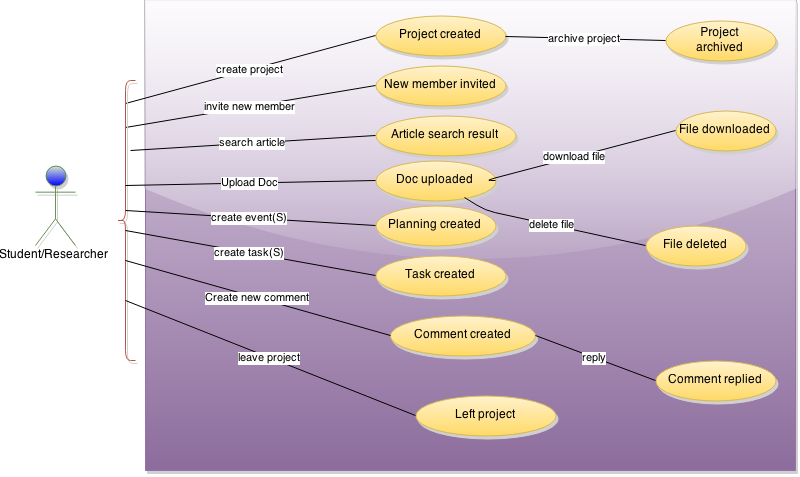
\includegraphics[scale=0.3]{./img/dsgn_img/USECASE1.png}	
\end{center}

% subsection subsection_name (end)

\subsubsection{Reviewer User} 
\begin{center}
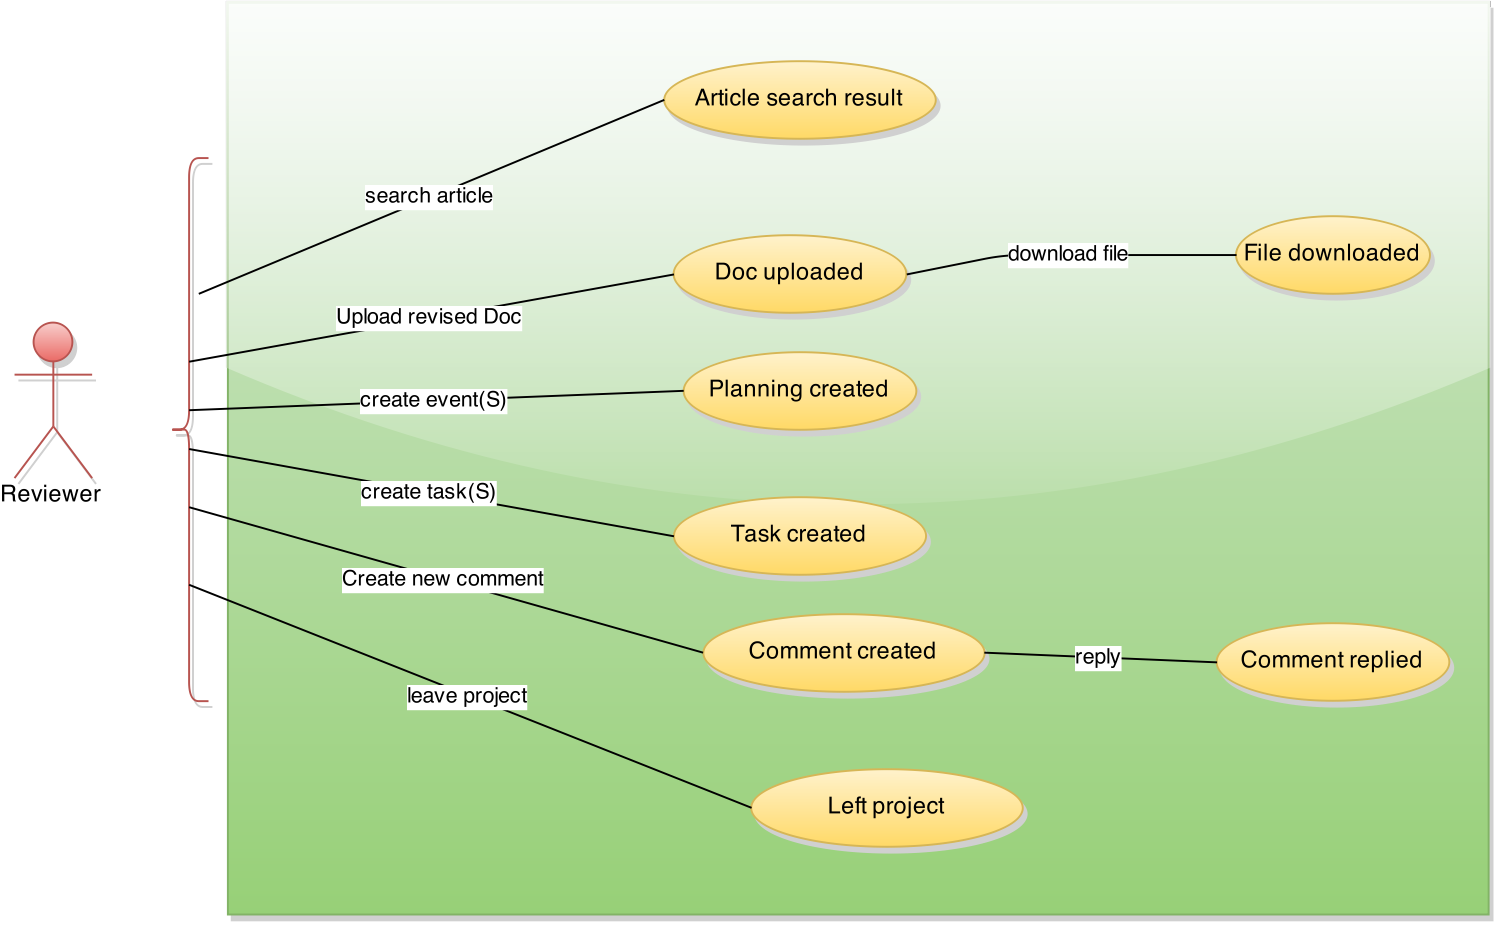
\includegraphics[scale=0.3]{./img/dsgn_img/USECASE2.png}
	
\end{center}

\subsubsection{Guest User} 
\begin{center}
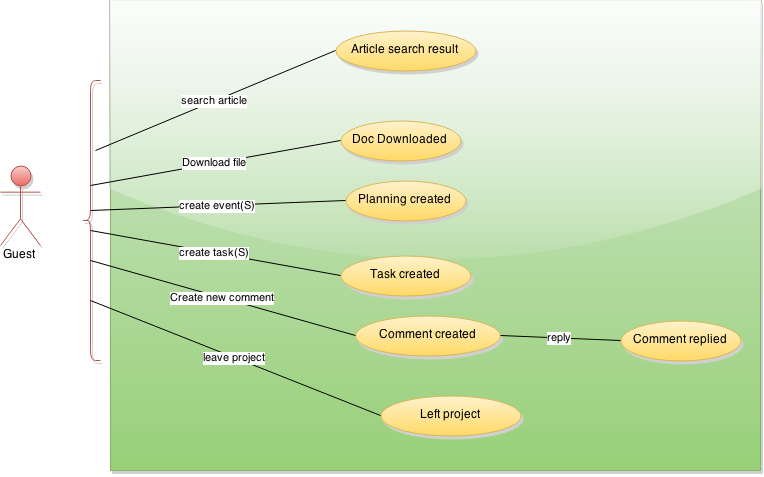
\includegraphics[scale=0.3]{./img/dsgn_img/USECASE4.png}
	
\end{center}

\subsubsection{Administrator User} 
\begin{center}
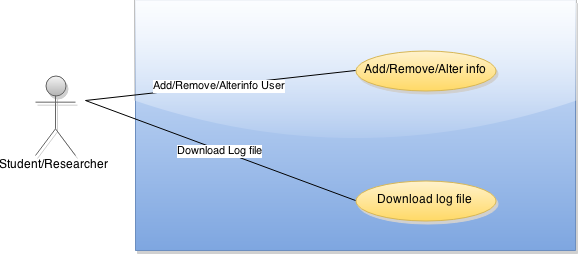
\includegraphics[scale=0.3]{./img/dsgn_img/USECASE3.png}
	
\end{center}
% subsection list_of_use_cases (end)

% subsection actors (end)
\newpage
\section{System Architecture} % (fold)
\label{sec:system_architecture}
For the purpose of modularity, the Model-View-Controller (MVC) design was adopted for the architecture of the application. In this section, the MVC
design of the system is illustrated in the form of a diagram. Its sub-components will also be discussed further down this section. MVC has been proven
to be very suitable for web architecture since it promises low coupling and high cohesion between components of the systems, and provides room for 
easier extension or modification of a specific component.
\subsection{Architectural Design} % (fold)
\label{sub:arichtectural_design}
%

In the app folder of this application, three packages are defined, corresponding to the MVC design. 
\begin{center}
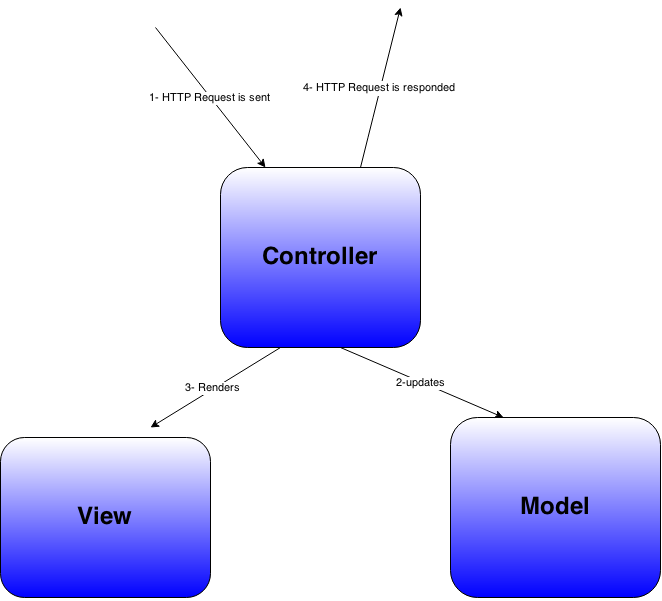
\includegraphics[scale=0.3]{./img/dsgn_img/MVCdiag.png}
	
\end{center}

The image above shows that the system architecture divides into three separate layers. The first layer is the model, which represents the information. 
The second layer is the view, which renders the information to the display of the user. The third and final layer is the controller, which interacts 
with user actions and processes them on the back-end accordingly. \\
In the next section we will explain each layer more thoroughly and explain the sub-components and their functions. 

\subsection{Model} % (fold)
\label{sub:design_rationale}
The model part of the design is meant to keep track of changes in the states of the application, such as (for example) when the user creates a new
project, or creates a new event in the calendar. When the user performs one of these actions, the model will propagate these changes from the 
views to the associated controllers within the application. The models also contain some operational methods that can be used (as static methods) to 
find or update information in the database.
\newpage
\subsubsection{Relational Model Diagram}

In order to give a more general overview of the system's model layer, a graphical representation of the Entity Relationship (ER) diagram is included to
show the relationships that the entities have with each other.

\begin{center}
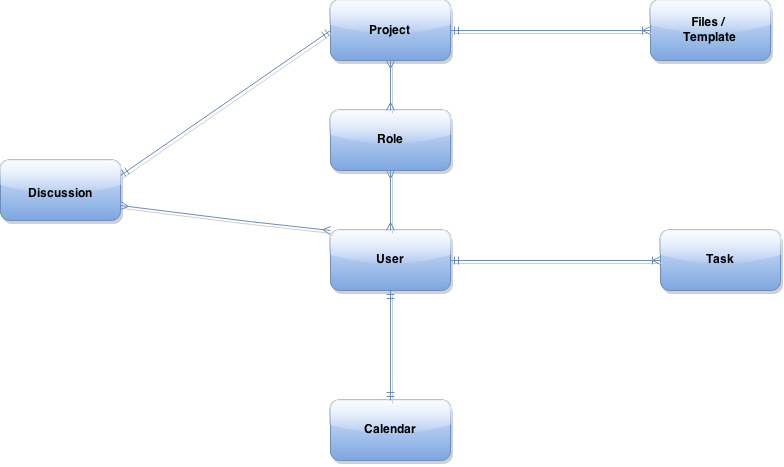
\includegraphics[scale=0.3]{./img/dsgn_img/RMA.png}
	
\end{center}

\subsubsection{Model description}
\paragraph{User}
The User model holds all the attributes a user needs within the application. Users are identified in the application by their (verified) email address 
which is unique. Almost all the models have a direct relation with the User model, as the user is a central component within the application. User 
attributes consist of an email, a name, etc.

\paragraph{Project}

The Project model is most likely the second most important model in this application, as many other models are also directly related to it. In fact, 
the entire application revolves around the user's interactions within a project. The main attributes that the Project model contains are the name of 
the project, the project creation date, the list of members and a few others.

\paragraph{Role}

The Role model is designed in order to distinguish what type of relation a user has to a project. The Role model holds the type of role a user has 
within a given project, the join date, and a boolean that indicates whether a User has either been invited, or has already confirmed the invitation. A
User can only take one role in the project at a time. 

\paragraph{Task} % (fold)
The Task model holds information about a task of a specific user. It keeps track of the name (can also be considered description), due date and a 
boolean variable that indicates whether a User has completed the task.

\paragraph{Calendar} % (fold)

The Calendar model holds information about an event for a user. An event is a basic part that builds up a planning for a project. It consist of a name,
a description, and a start and end date. 

\paragraph{Discussion} % (fold)
Members of a project should be able to discuss issues about their project. The Discussion model is designed to keep track of relevant data concerning a 
discussion. It contains a subject and description, with a time stamp to keep track of when a message has been posted. 

\paragraph{Document Files} % (fold)
The Document file model holds information about the version and name of a specific file that is uploaded into a project. Any file that is uploaded is 
assigned a unique version number, meant to identify files with the same name in the same project. It also contains the data of the user that uploaded
the file, and a link to where the uploaded file is stored.

\paragraph{Mendeley Document} % (fold)
The Mendeley Document model is meant to store the meta data retrieved from user's Mendeley libraries. Its main attribute the is JSON data
stored as a String so that the application can easily push the same data to another user's Mendeley library. Some other attributes such as
title, type and authors are copied from this JSON to make searching for specific files easier.

\subsection{View} % (fold)
The View part of the MVC architecture is the gate for the user to interact with the application. The View layer is designed to be simple
and minimalistic. An image snapshot of the view's sub-components are shown next.
\subsubsection{Login}

\begin{center}
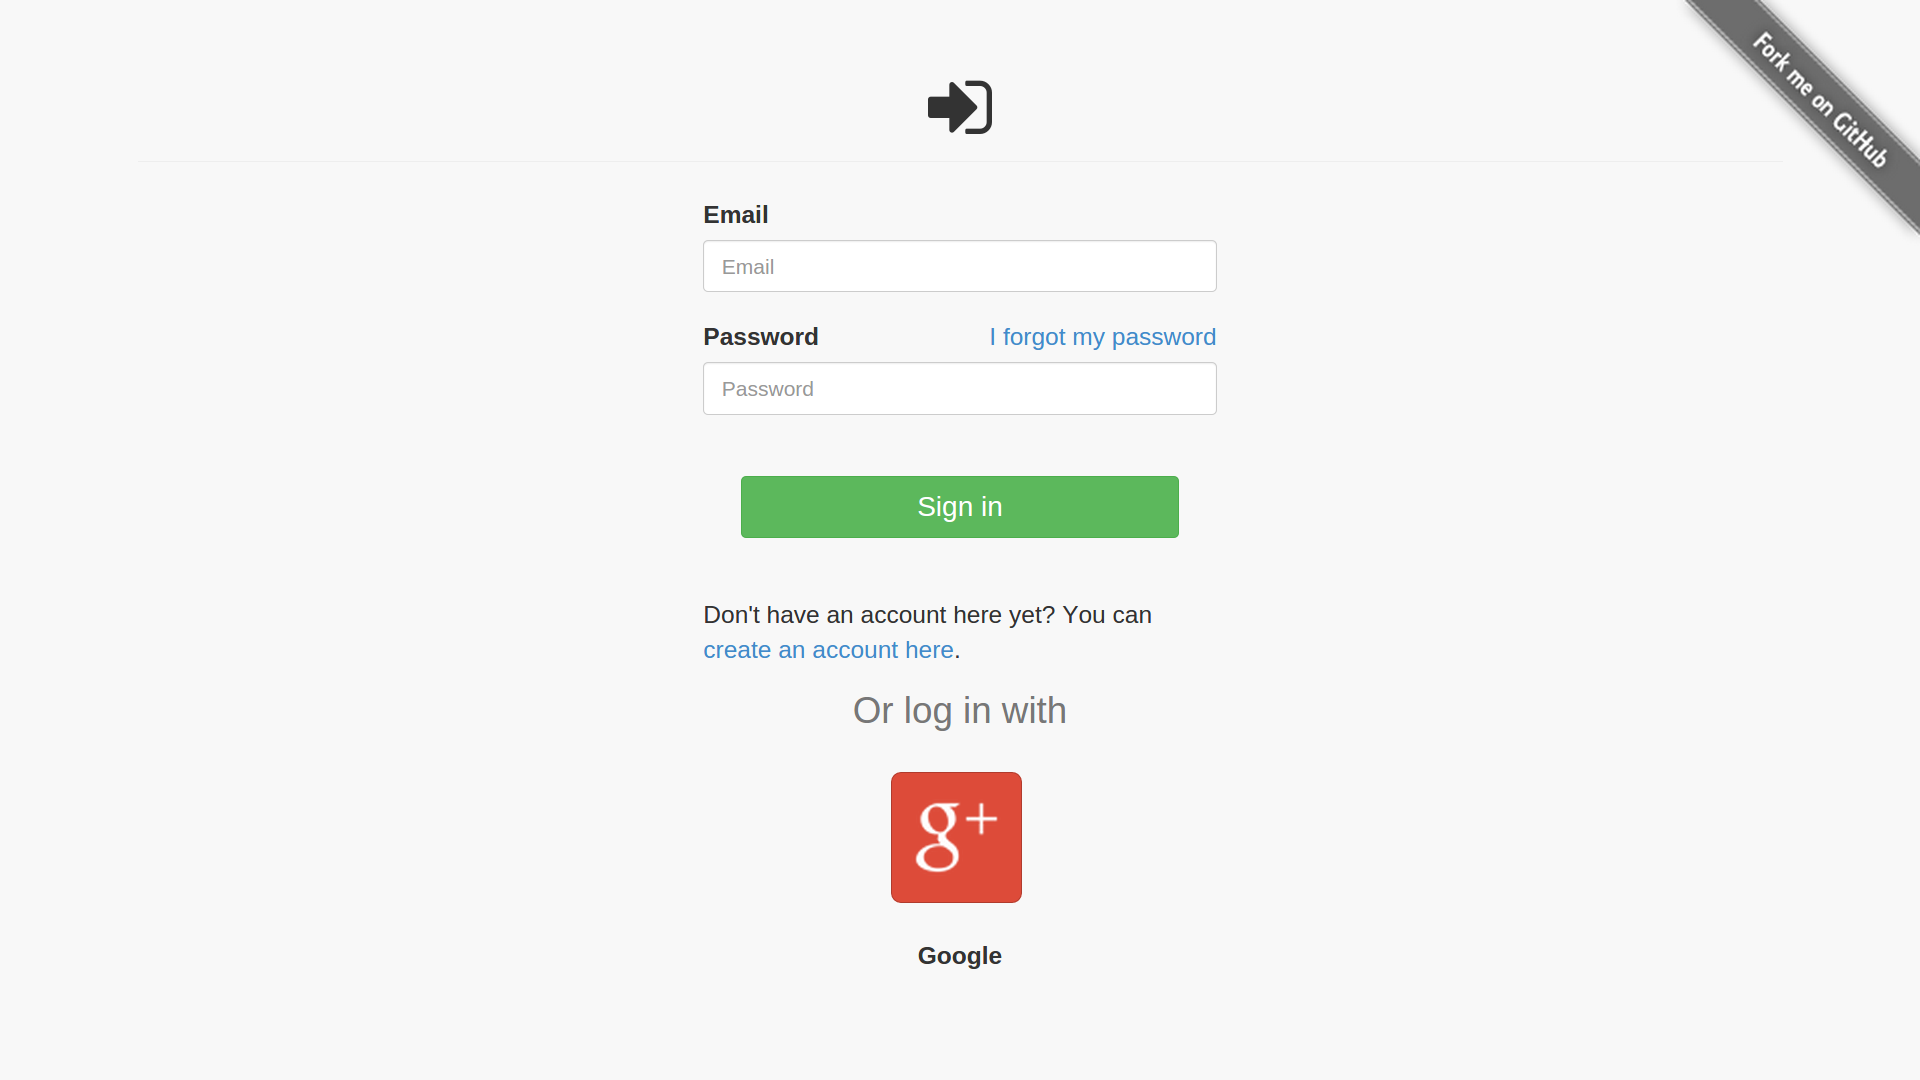
\includegraphics[height=200px, width=350px]{./img/dsgn_img/login.png}
	
\end{center}

\subsubsection{Dashboard}

\begin{center}
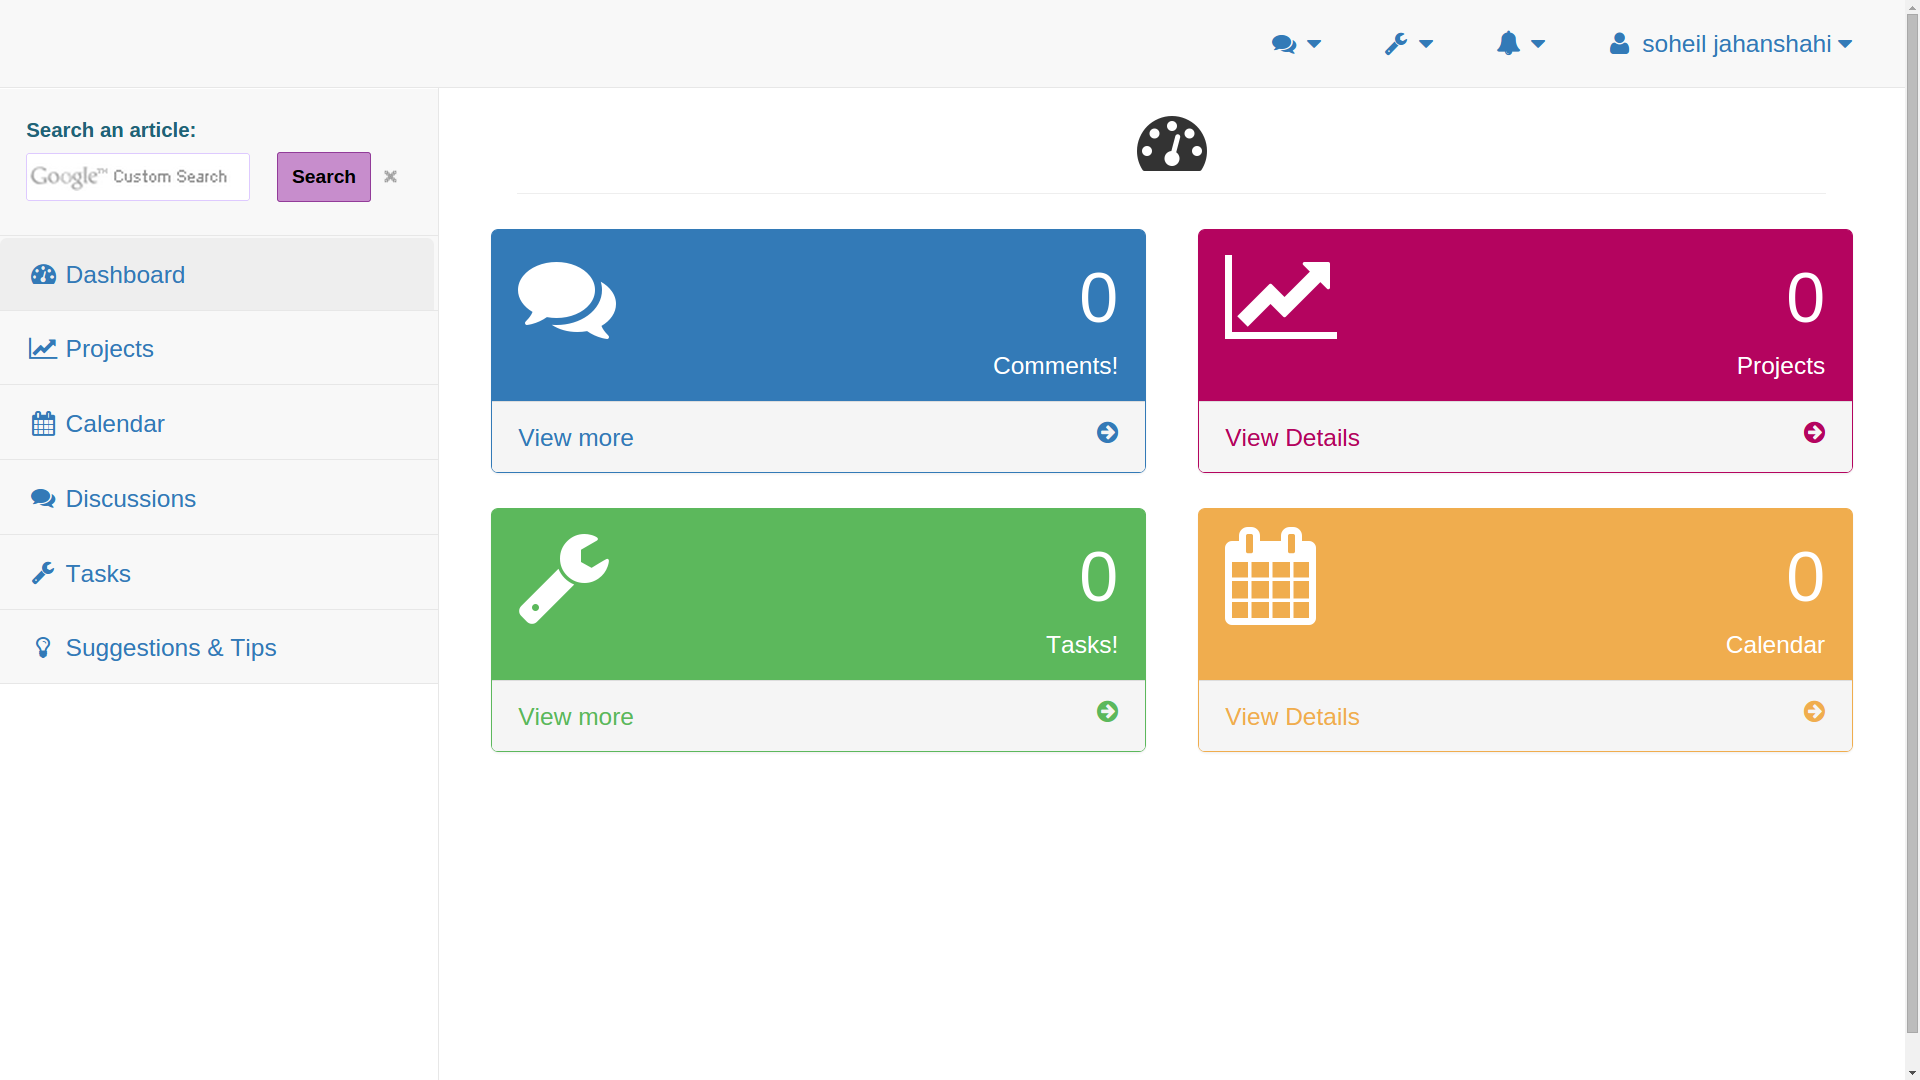
\includegraphics[height=200px, width=350px]{./img/dsgn_img/dashboard.png}
	
\end{center}

\subsubsection{Project}

\begin{center}
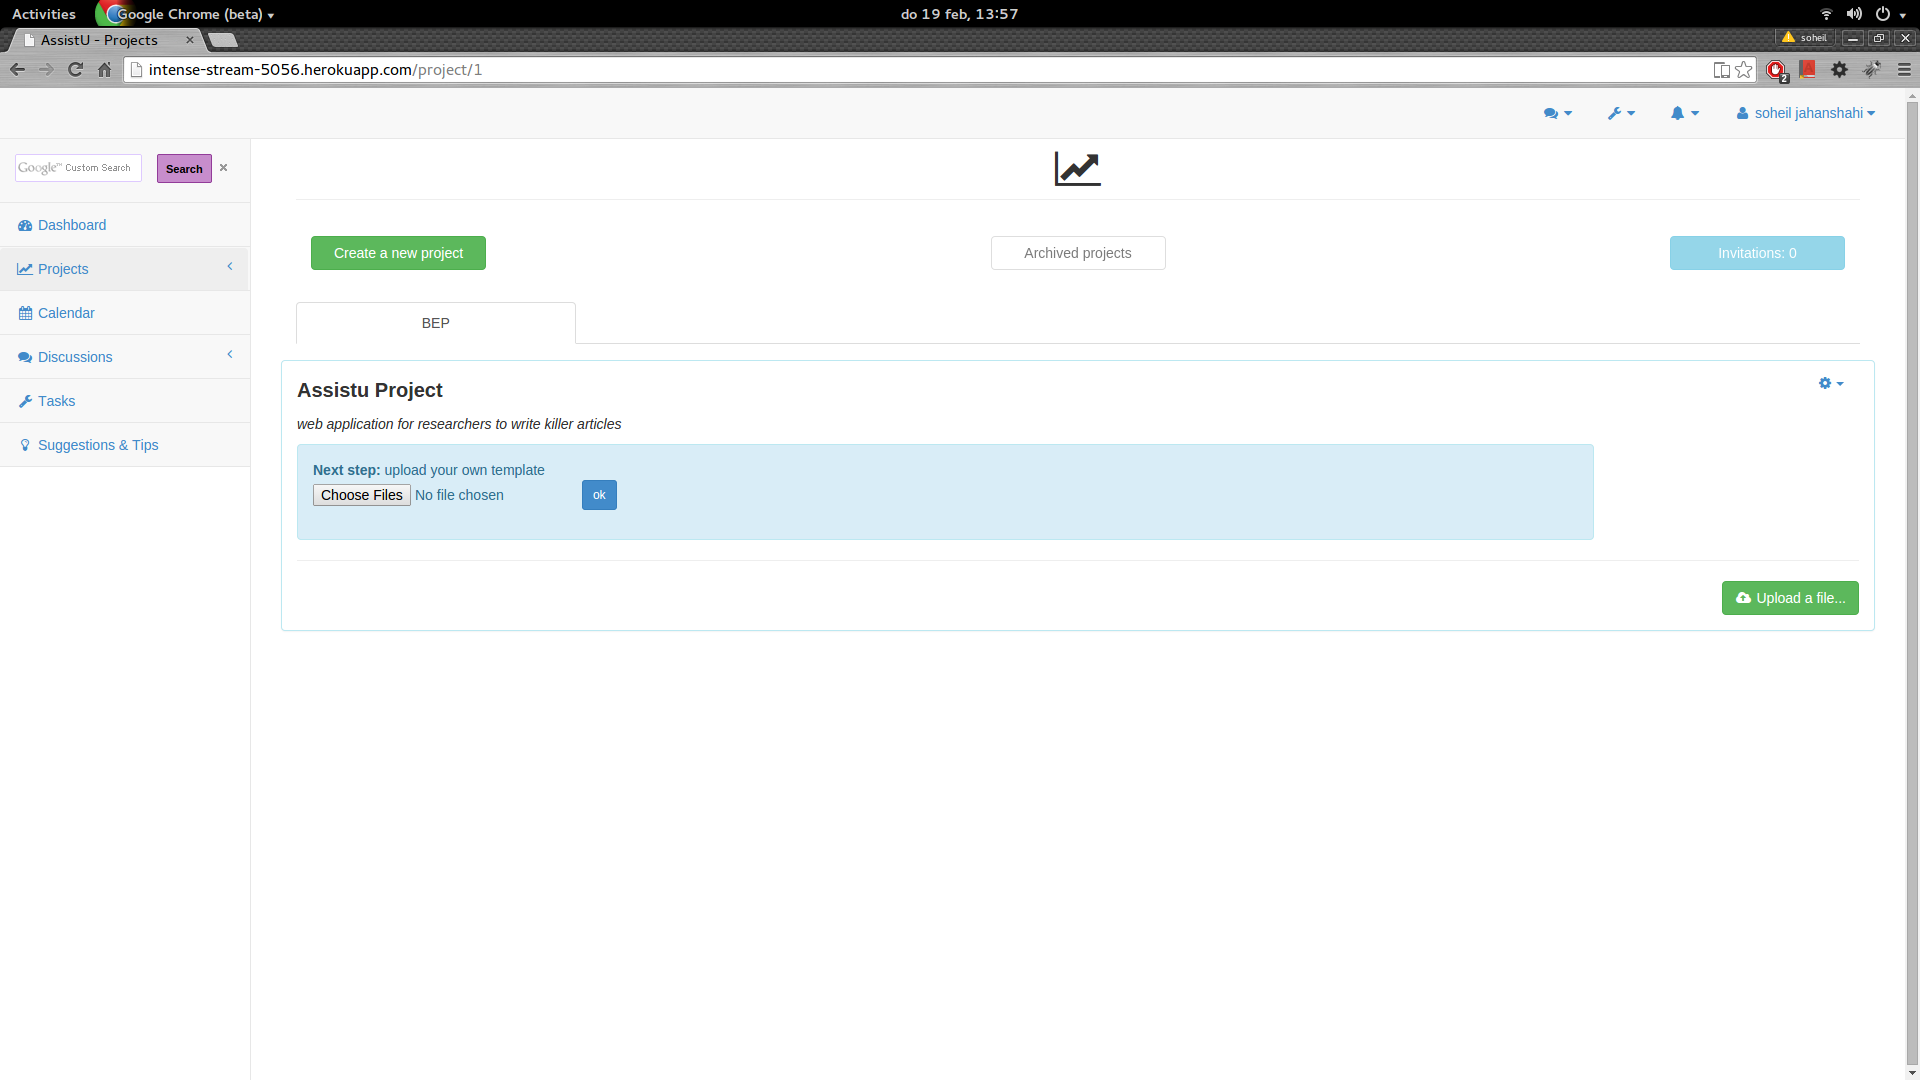
\includegraphics[height=200px, width=350px]{./img/dsgn_img/project.png}
	
\end{center}
\subsubsection{Discussion}

\begin{center}
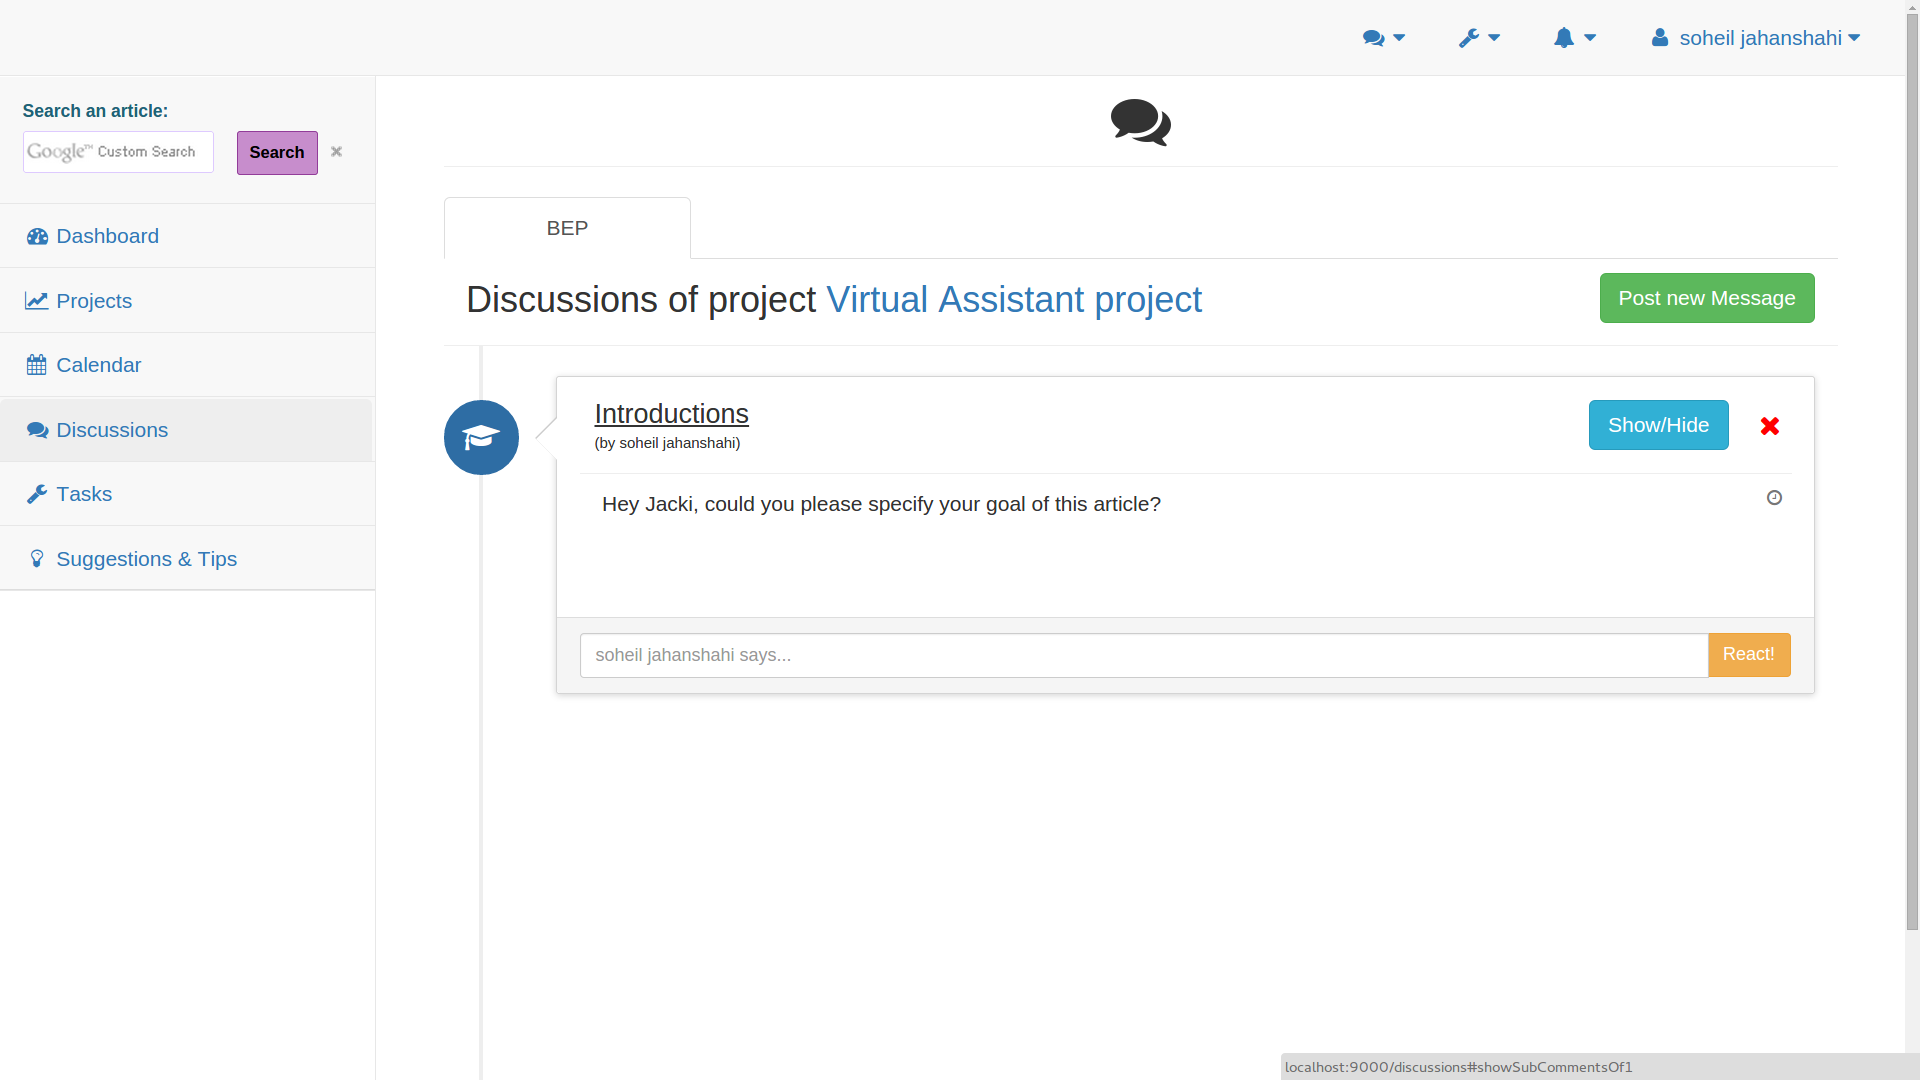
\includegraphics[height=200px, width=350px]{./img/dsgn_img/discussion.png}
	
\end{center}

\subsubsection{Calendar}

\begin{center}
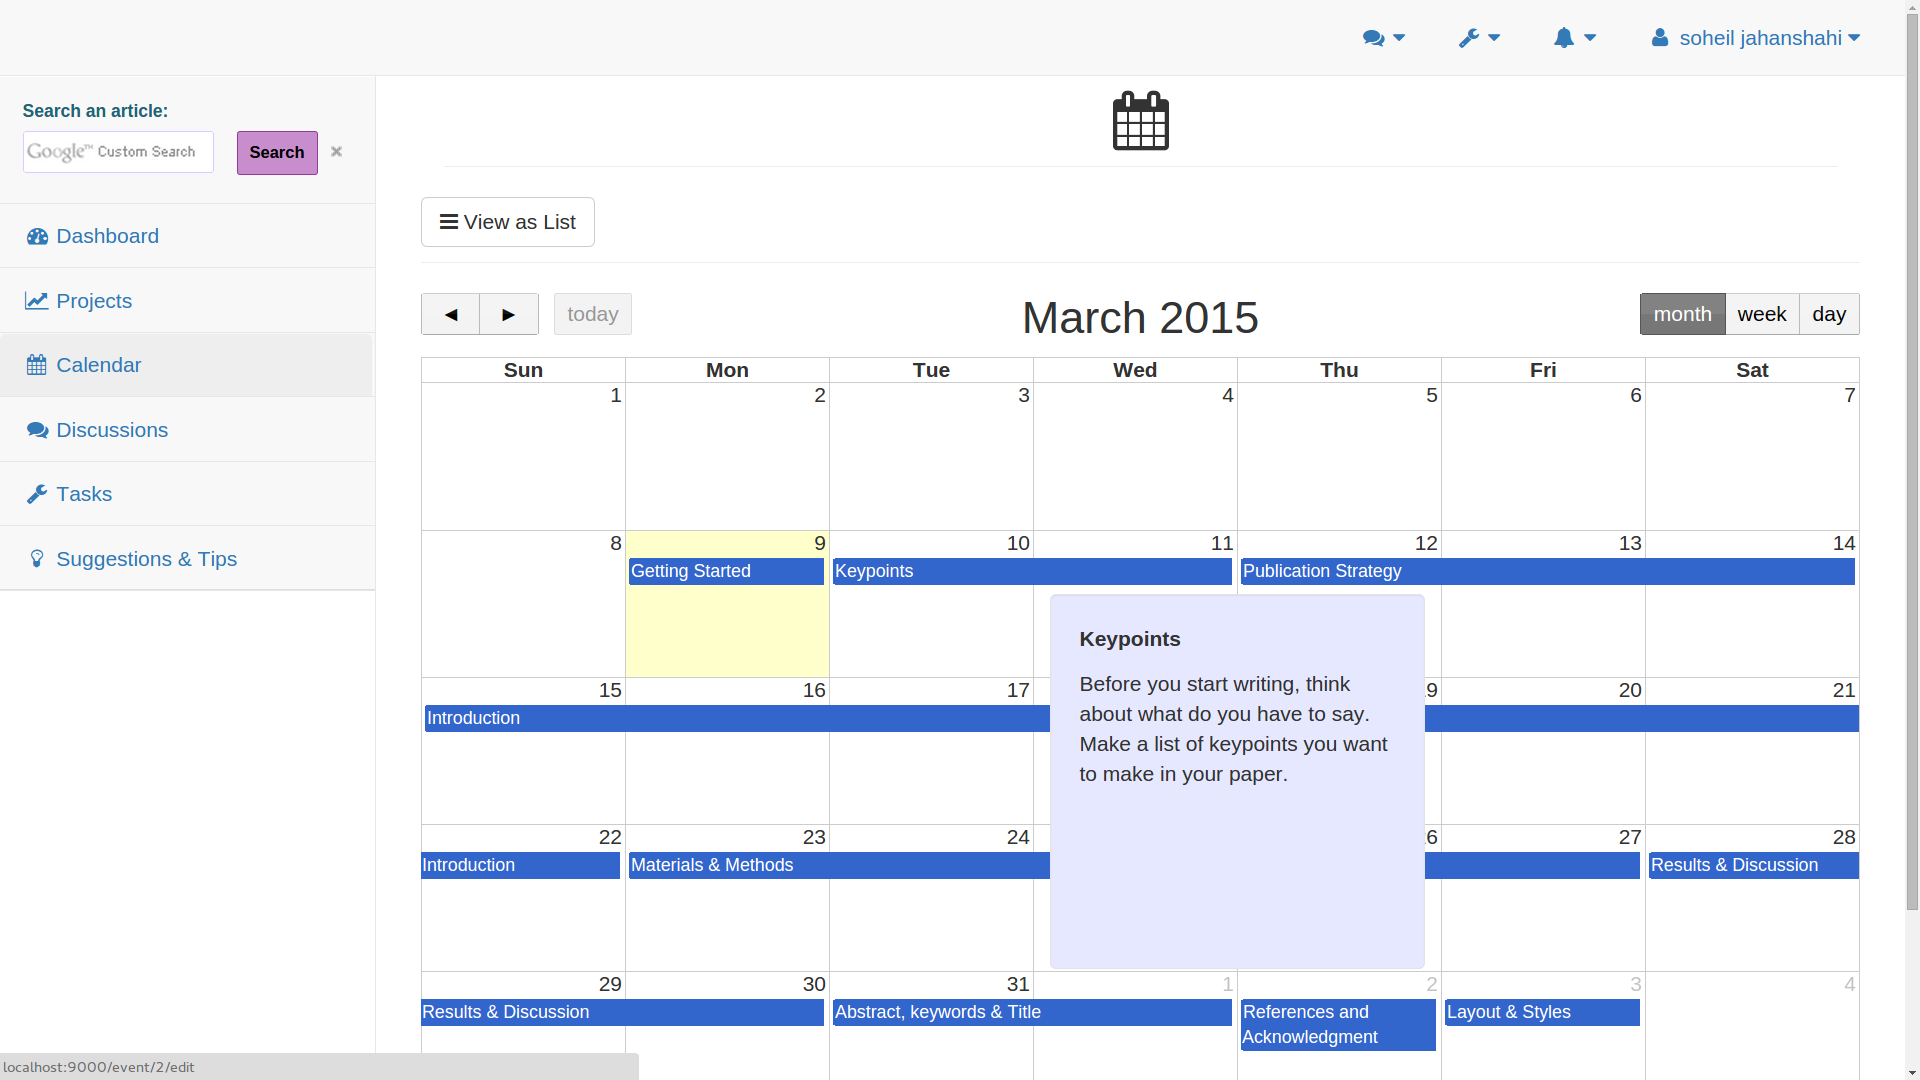
\includegraphics[height=200px, width=350px]{./img/dsgn_img/calendar.png}
	
\end{center}

\subsubsection{Task}

\begin{center}
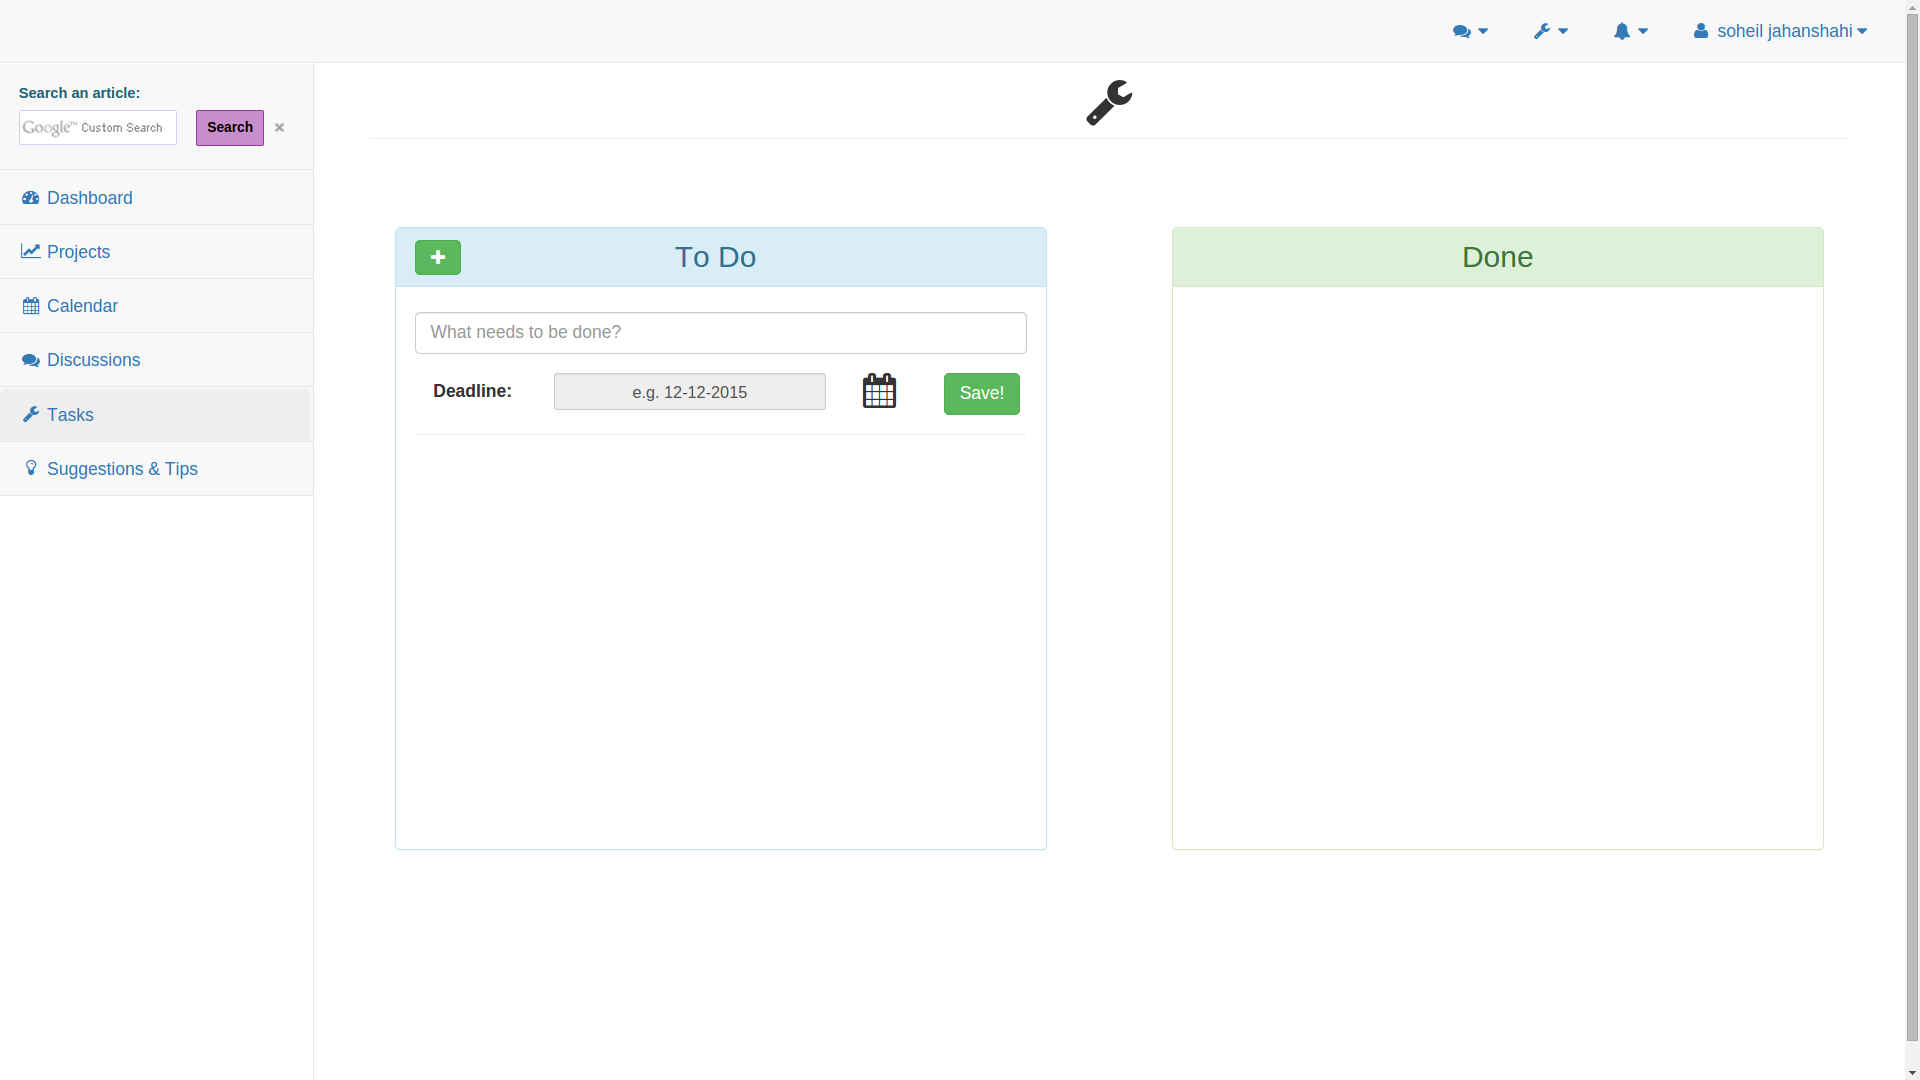
\includegraphics[height=200px, width=350px]{./img/dsgn_img/task.png}
	
\end{center}

\subsubsection{Suggestions}

\begin{center}
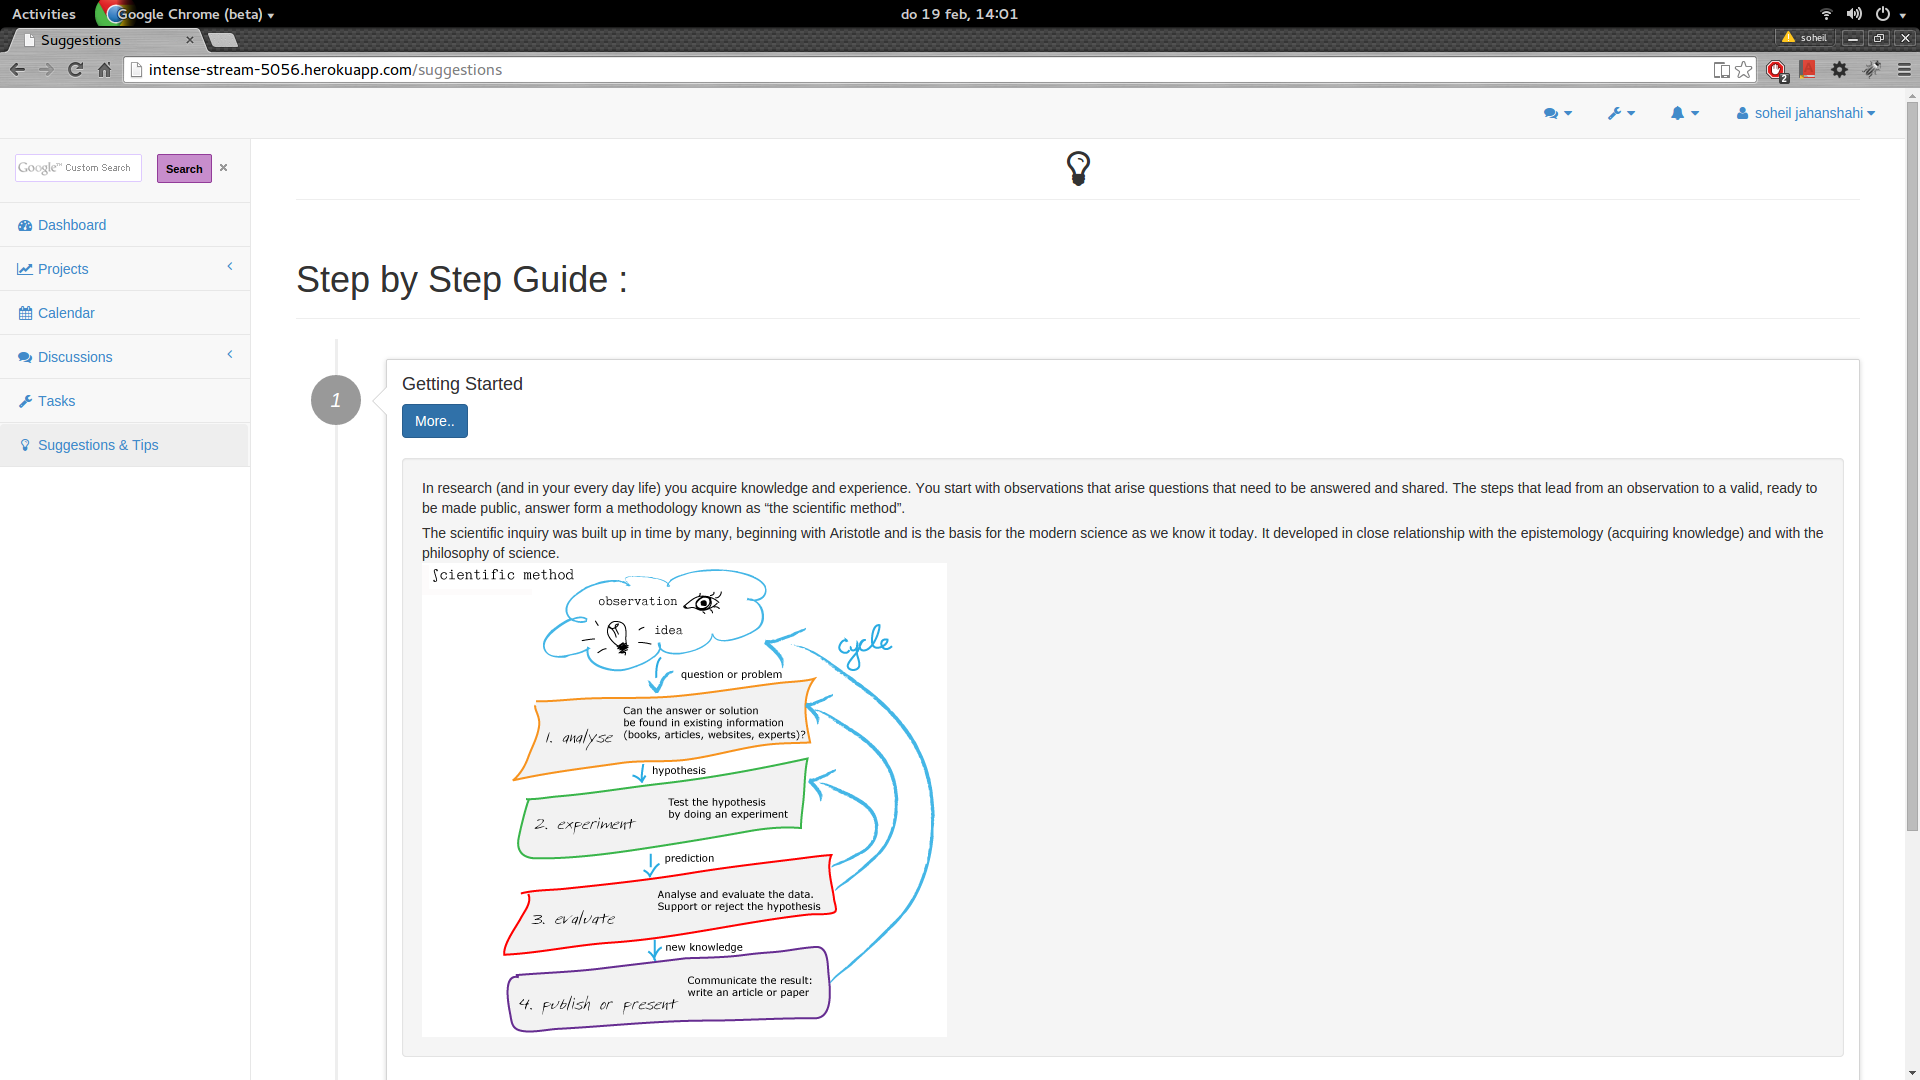
\includegraphics[height=200px, width=350px]{./img/dsgn_img/suggestions.png}
	
\end{center}
\newpage
\subsection{Controller}
The Controllers are the brains of the application. They handle all the requests committed by users from the view part, and respond to it accordingly.\\
The Controllers are also responsible to update the models if there is any change in the state of the information. In the table below an overview of all controllers with their responsibility is shown.\\

\begin{center}
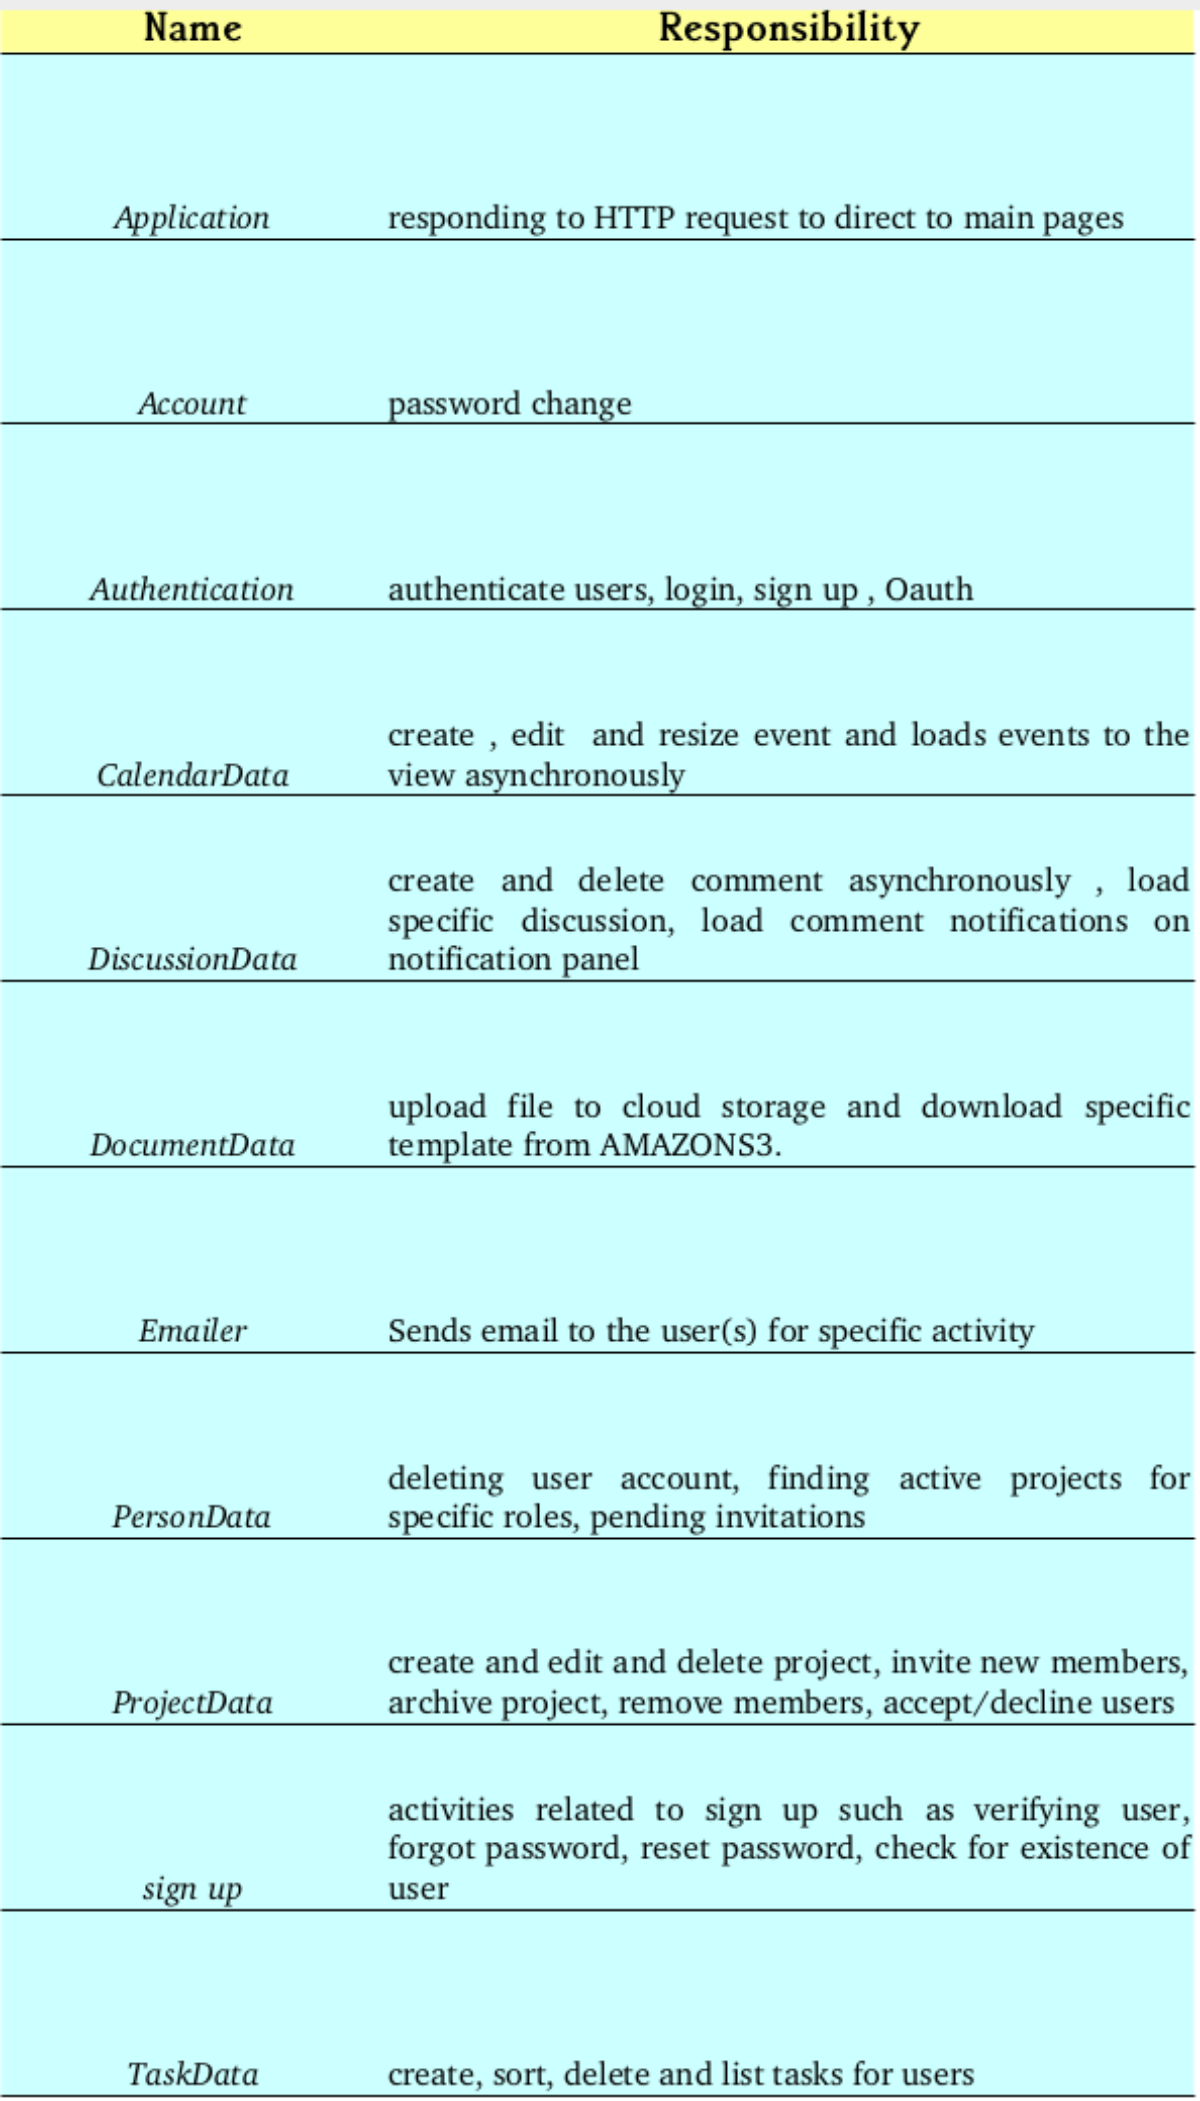
\includegraphics[height=300px, width=300px]{./img/dsgn_img/controllers.png}
	
\end{center}